In this section, we introduce the model transformation language DSLTrans which is at the heart of our technique.

\subsection{The DSLTrans Transformation Language}


DSLTrans is a visual graph-based and rule-based model
transformation engine that has two important properties enforced by construction: all its computations
are both \emph{terminating} and \emph{confluent}~\cite{Barroca2011}.
These properties stem from the fact that DSLTrans does not allow
unbounded loops during execution, making it a Turing-incomplete
computing language~\cite{Barroca2011}. Besides their obvious importance in
practice, \emph{termination} and \emph{confluence} were instrumental in the
implementation of our verification technique for pre-/post-condition contracts.

Note that to provide this verification ability, it is not possible to delete elements in DSLTrans, and all input models must be finite. Despite the apparent lack of expressivity, our experience has showed that it is
possible to specify a wide range of transformations using DSLTrans, including a previous industrial example~\cite{Selim2014} and the case study discussed in Section~\ref{sec:mbeddr_transformation}.

Model transformations are expressed in DSLTrans as sets of graph rewriting
rules, having an upper part (named \emph{MatchModel}), a lower part (\emph{ApplyModel}) and,
optionally, negative application conditions.

The main construction used in the scheduling of DSLTrans model transformation rules is a
\emph{layer}. These layers are in a particular order, and each contains a set of \emph{rules}. The rules inside the same layer are executed independently of one another, i.e., there is no order of execution of rules, and each rule in a layer cannot match over the output of any other rule in the same layer. As well, rules cannot modify the input graph during the rewriting phase (termed \emph{out-place} execution). Layers are organized sequentially and therefore the output model that results from executing a given layer is passed as input to
the next layer in the sequence.

A DSLTrans rule can match over the elements of the input model of the
transformation and also over elements that have been generated so far in the
output model. Matching over elements of the output model of a
transformation is achieved using a DSLTrans construct called \emph{backward
links}. Backward links allow matching over traces between elements in the input and
the output models of the transformation. These traces are explicitly built by
the DSLTrans transformation engine during rule execution.

 \begin{figure}[t]
   \begin{center}
     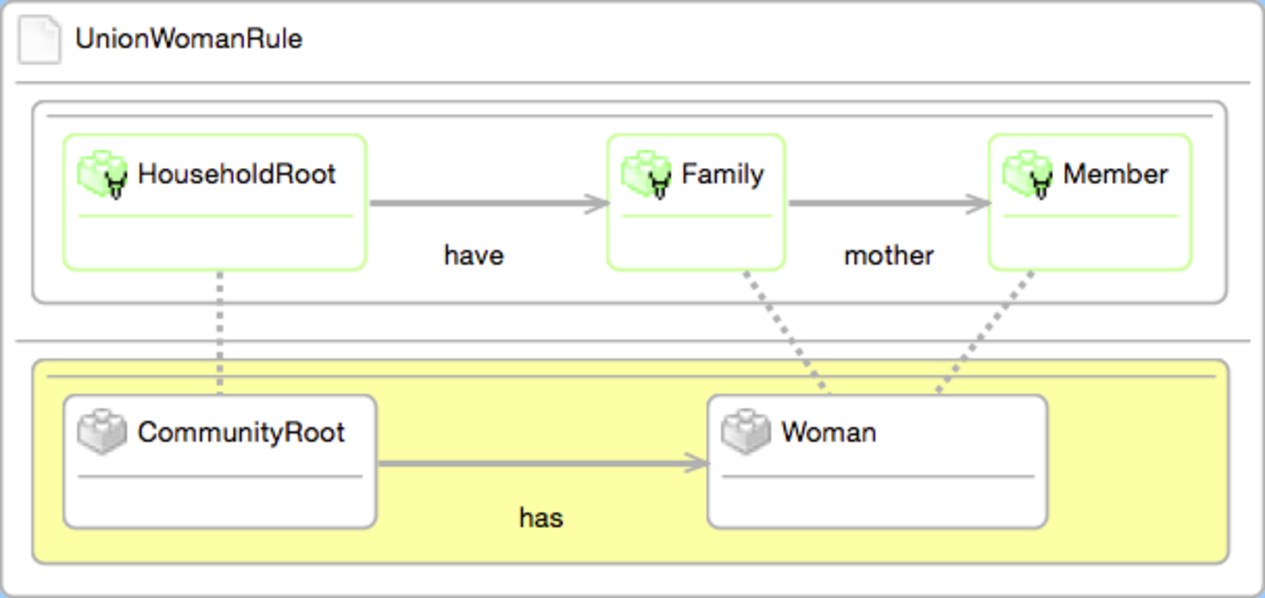
\includegraphics[width=0.40\textwidth]{figures/FamToPersons/UWRule}
     \caption{An example of a DSLTrans rule}
     \label{fig:DSLTrans_rule}
   \end{center}
   \vspace{-0.25in}
 \end{figure}

For example, we depict in Figure~\ref{fig:DSLTrans_rule} a
rule in the DSLTrans language.
When a rule is executed, the graph in the \emph{MatchModel} of the rule is searched for in the transformation's input model, together with the classes in the \emph{ApplyModel} of the rule that are connected to \emph{backward
links}. An example of a \emph{backward link} can be observed in
Figure~\ref{fig:DSLTrans_rule} as a dotted line connecting the \emph{Country} and the
\emph{Community} match classes. During the rewrite part of rule application,
the instances of classes in the \emph{ApplyModel} of the rule that are not connected to
backward links, together with their adjacent relations, are created in the
output model.

For example, the \emph{UnionWomanRule} rule in Figure~\ref{fig:DSLTrans_rule} will match over a \emph{Country} element connected to a \emph{Family} element connected to a \emph{Parent} element. If these elements are found in the input model along with the corresponding \emph{Community} and \emph{Woman} elements in the output model, then a \emph{persons} relation will be created between those output elements.

Although not present in this rule,
copying object attribute values from the \emph{MatchModel} to the \emph{ApplyModel} of the rules is
also part of the DSLTrans language, as illustrated in Section~\ref{sec:DSLTransRepresentation}.


In addition to the constructs presented in the example in
Figure~\ref{fig:DSLTrans_rule}, DSLTrans has several others:
\emph{existential matching} which allows selecting only one result when a match class of a rule
matches an input model, \emph{indirect links} for transitive matching
over containment relations in the input model, and \emph{negative application
conditions} that allow the transformation designer to specify conditions under
which a rule should not match. These constructs are not currently used in
our verification approach, and the interested reader is referred to~\cite{Barroca2011} for further information.


\subsection{Families-To-Persons Example}

As our introductory example to the syntax and semantics of DSLTrans, we present the \FTP transformation previously described in \cite{Oakes2016}. The original \FTP transformation can be
found in the ATL zoo~\cite{atlZoo}, and has also been discussed in a number of related works on verification and testing~\cite{Gogolla2011}.

We chose this \FTP transformation as our introductory example as it translates between easily-understood domains, as described below.

\begin{figure}[bt]
\centering
\subfigure[\emph{Families\_Extended} metamodel]{
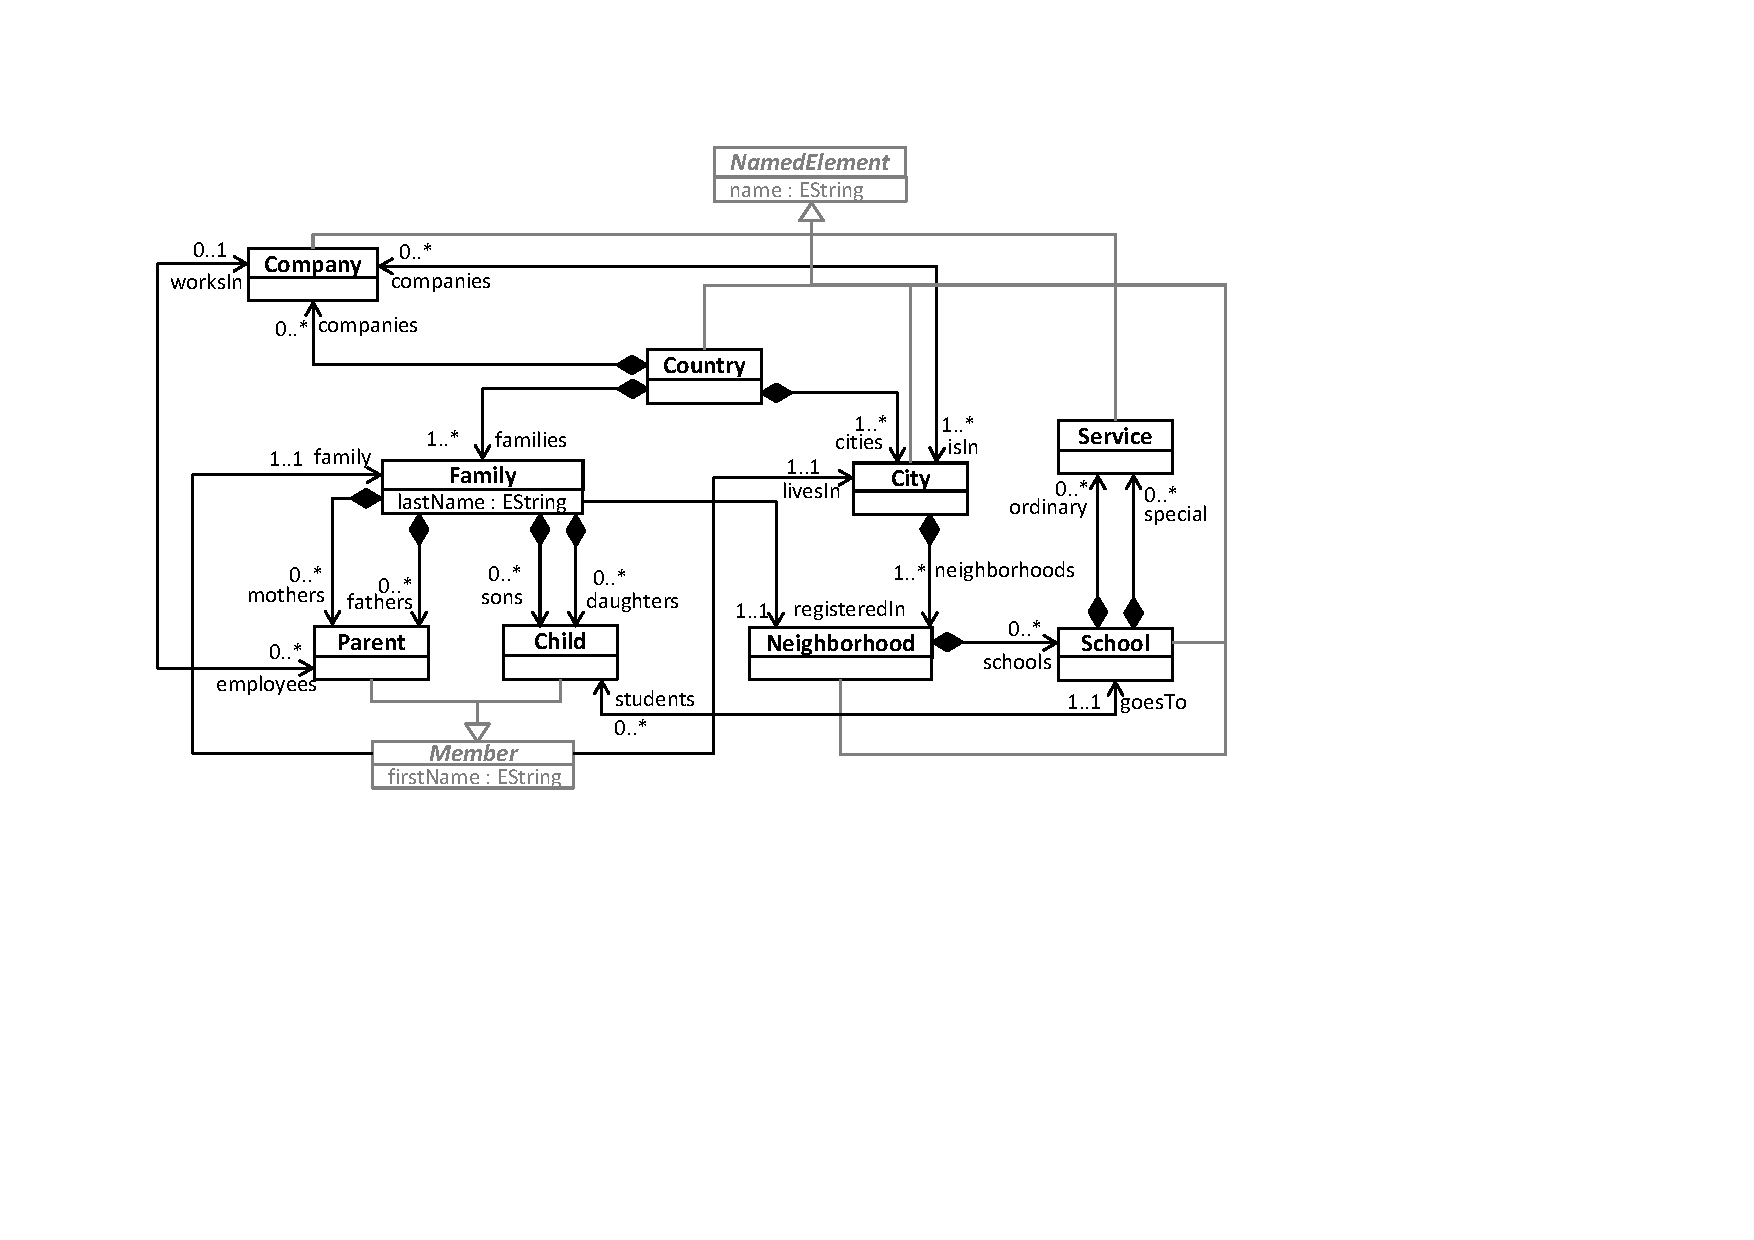
\includegraphics[width=0.97\columnwidth]{figures/FamToPersons/Families_Extended.pdf}
\label{fig:fams}
}
\subfigure[\emph{Persons\_Extended} metamodel]{
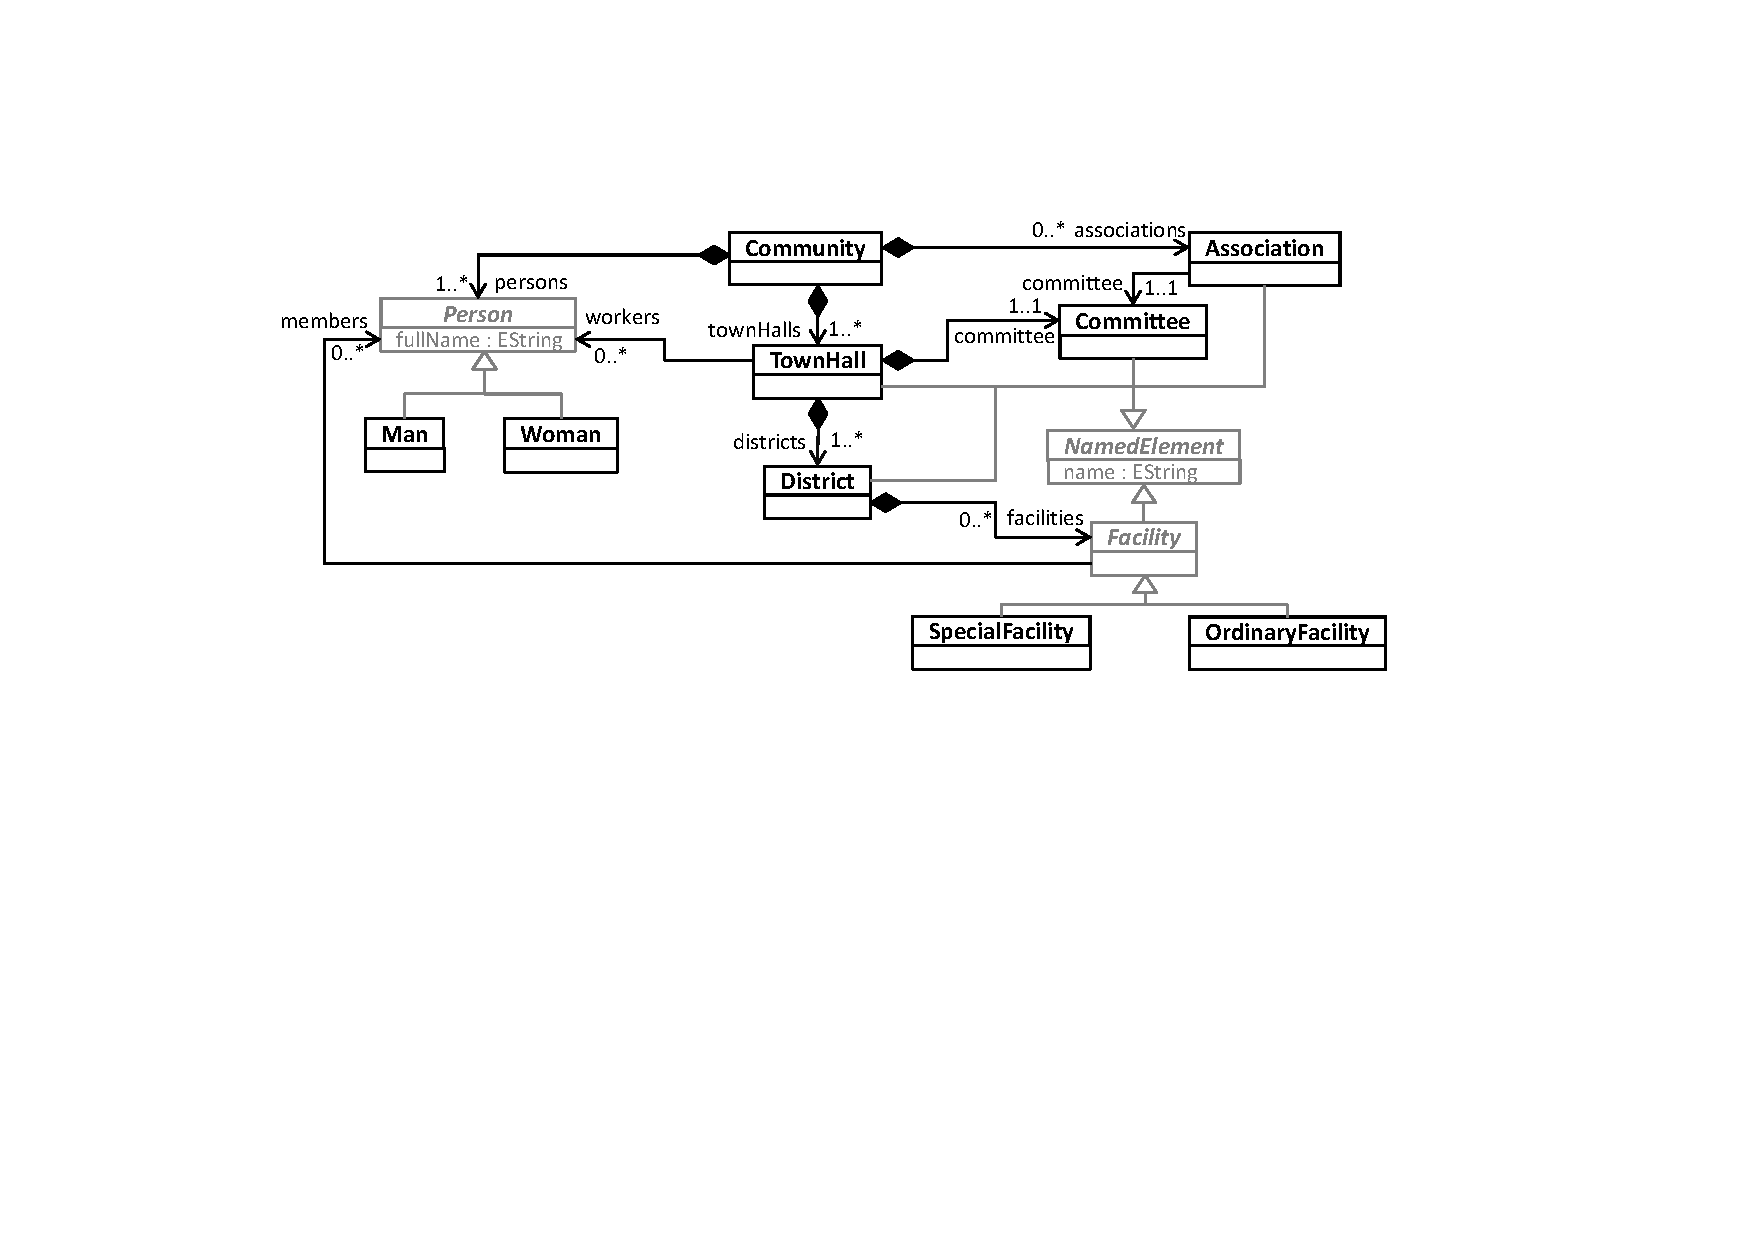
\includegraphics[width=0.97\columnwidth]{figures/FamToPersons/Persons_Extended.pdf}
\label{fig:pers}
}
\caption{Metamodels of the \emph{Families-to-Persons\_Extended} transformation}\label{fig:metamodels}
\end{figure}

The input and output metamodels of this transformation are shown in Figure~\ref{fig:metamodels}. Please note that abstract classes are depicted in grey color and with italic names, and inheritance relationships are depicted in grey.

The input metamodel, the \emph{Families\_Extended} metamodel, has the \emph{Country} class as a root element.
A \emph{Country} is made up of \emph{companies}, \emph{families} and \emph{cities}.
A \emph{Family} has a \emph{lastName}, is \emph{registeredIn} a \emph{Neighborhood} and can have any number of \emph{mothers} and \emph{fathers}, who are \emph{Parent}s and may, in turn, work in (\emph{worksIn}) a \emph{Company}.
It can also contain any number of \emph{sons} and \emph{daughters}, who are \emph{Child}ren, and every child \emph{goesTo} a \emph{School}.
Both parents and children are \emph{Member}s that have a \emph{firstName}, belong to a \emph{family} and each of them \emph{livesIn} a \emph{City}.

A \emph{City} may contain \emph{companies}, and a \emph{Company}, in turn, can be present in (relationship \emph{isIn}) several distinct cities.
A \emph{City} is composed of \emph{neighborhoods}, and these can have \emph{schools}, where several \emph{students} are registered.
Every \emph{School} has \emph{Service}s, and these may be \emph{special}, for students with special needs, or simply offer \emph{ordinary} services.
Finally, countries, cities, companies, neighborhoods and schools have a \emph{name} attribute, which is inherited from the abstract \emph{NamedElement} class.

The output metamodel, \emph{Persons\_Extended}, is shown in Figure~\ref{fig:pers}.
The root class is \emph{Community}, which is made up of \emph{persons}, \emph{townHalls} and \emph{associations}.
A \emph{Person} has a \emph{fullName} and can either be a \emph{Man} or a \emph{Woman}.
An \emph{Association} has a \emph{Committee} that makes decisions.
Every \emph{TownHall} has a roster of \emph{workers} (all the persons that are employed), hosts a \emph{Committee} to make decisions, and also governs several \emph{districts}.
A \emph{District} may contain several \emph{facilities}, either of type \emph{SpecialFacility} for those with special needs, or \emph{OrdinaryFacility}.
Each \emph{Facility} may have registered several persons as \emph{members}.
Finally, associations, town halls, committees, districts and facilities have a \emph{name} attribute.


\subsection{DSLTrans Representation}\label{sec:DSLTransRepresentation}

\begin{figure*}
  \begin{center}
  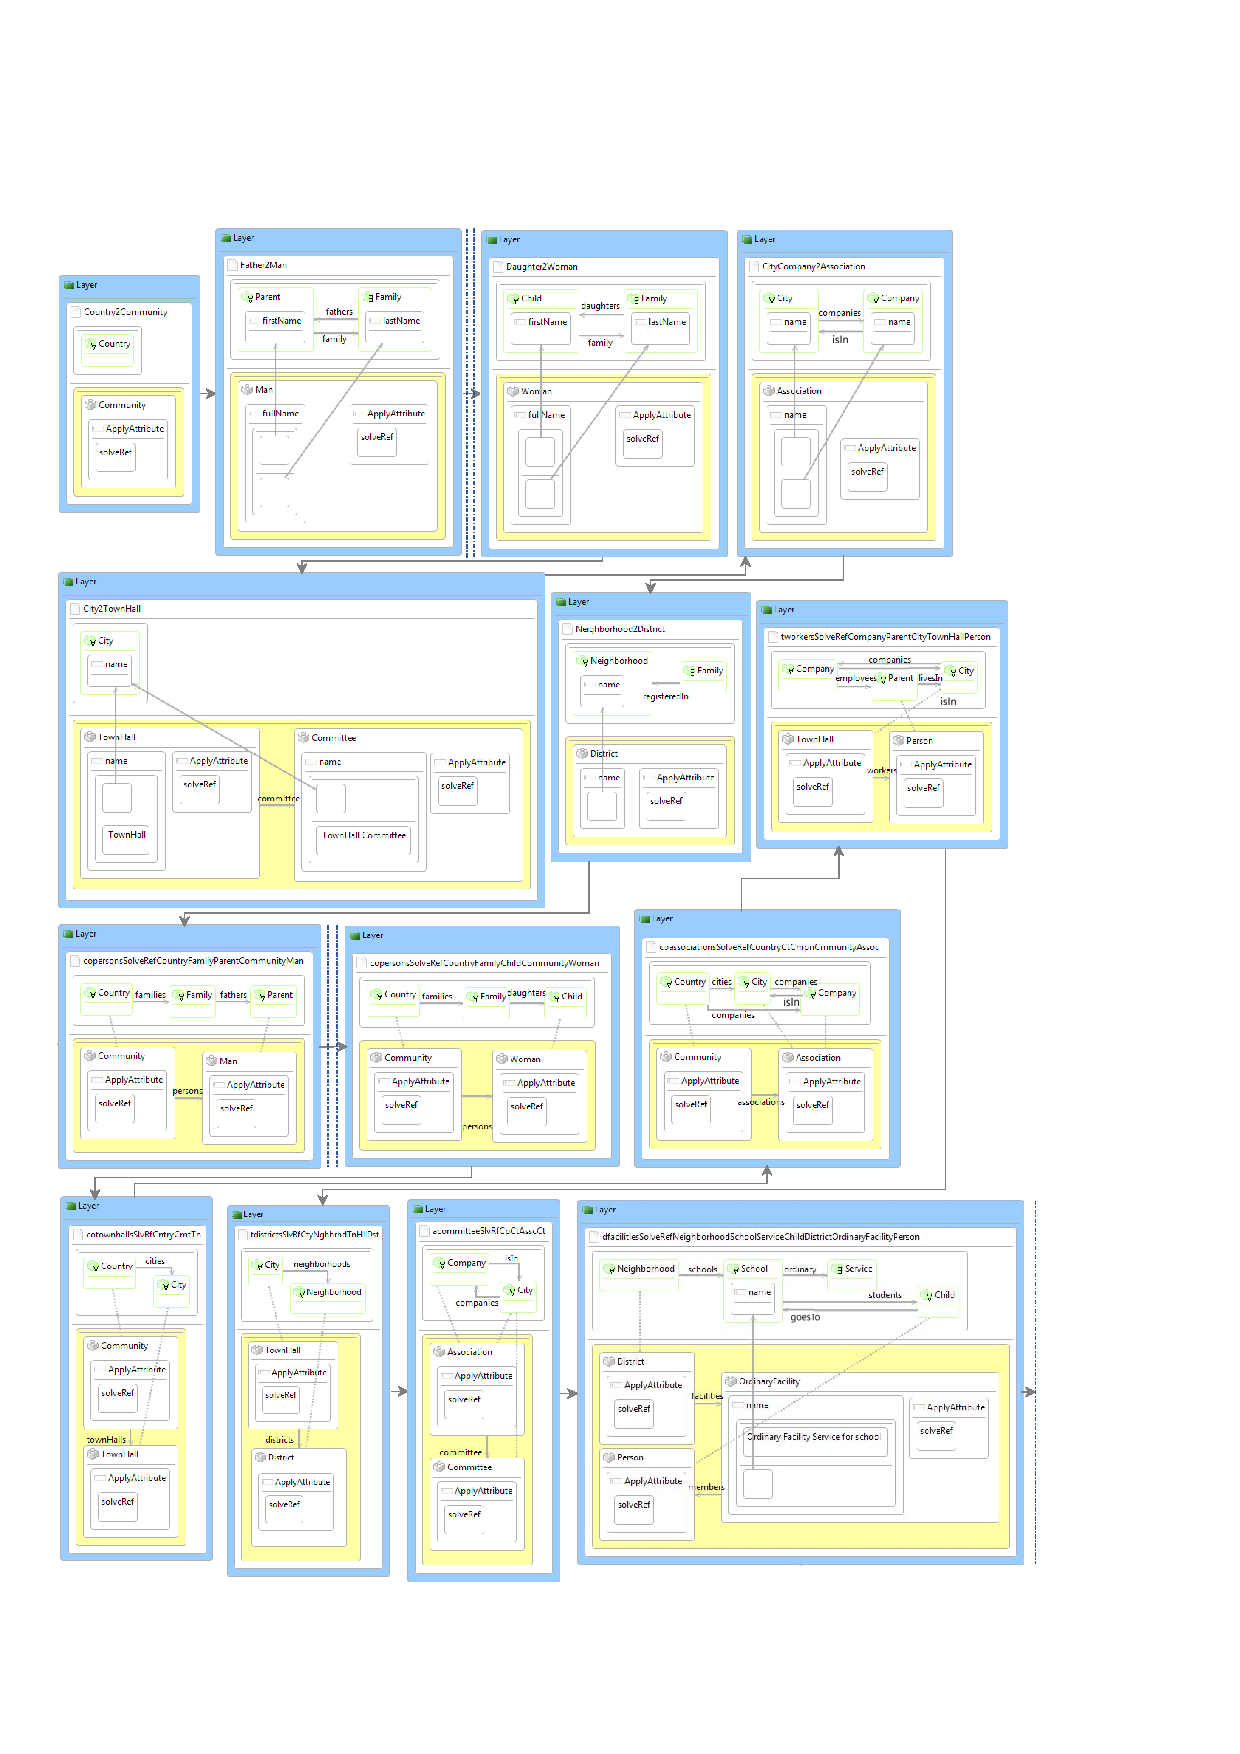
\includegraphics[width=0.94\textwidth]{figures/FamToPersons/DSLTrans_Rules_javi}
  \caption{DSLTrans version of the \emph{Families-to-Persons\_Extended} transformation}
  \label{fig:DSLTrans_rules}
  \end{center}
\end{figure*}


Figure~\ref{fig:DSLTrans_rules} displays the Families-To-Persons DSLTrans transformation . Let us mention here that we have removed five rules from the figure to improve visual clarity.
There is a vertical dotted blue line for each of these rules, located where the rules have been removed. The missed rules are similar to those that surround them, and can therefore be safely ignored in our explanation.

Note that this DSLTrans transformation has been automatically created from a declarative ATL version, as discussed in~\cite{Oakes2016}. This is the reason that only one rule is in each layer.

The first six rules shown in Figure~\ref{fig:DSLTrans_rules} are those that create elements in the output model whenever their MatchModel is found in the input model. The following eight rules presented connect those elements with associations, where the elements to be connected are found by backward links.

For example, the rule \emph{Country2Community} will create a \emph{Community} element for every \emph{Country} in the input model. The rule \emph{Daughter2Woman} will match over a \emph{Child} element connected to a \emph{Family} using a \emph{daughters} association, and produce a \emph{Woman} element. Then, the rule \emph{copersonsSolveRefCountryFamilyChildCommunityWoman}\footnote{The names were automatically generated by the higher-order transformation.} will link the \textit{Woman} to the appropriate \textit{Community} using a \textit{has} association. Note that the appropriate elements are determined by the backward link connecting the \emph{Community} and \emph{Country} elements, as well as the backward link connecting the \emph{Child} and \emph{Woman} elements. 


Note that attribute copies are represented with arrows from the \emph{ApplyModel} of the rule to the \emph{MatchModel}, such as in rule \emph{Neighborhood2District}, where the created \emph{District} gets the same name as the matched \emph{Neighborhood}.
The string of an attribute of a created element can also be initialized with the concatenation of several strings.
For instance, in rule \emph{Father2Man}, the full name of the created \emph{Man} comes from the concatenation of the first name of the matched \emph{Parent} and the last name of his/her \emph{Family}.
Or it can be assigned the string of an attribute of an element in the \emph{MatchModel} concatenated with a given string, such as in rule \emph{City2TownHall}.


%\emph{Father2Man} in Figure~\ref{fig:DSLTrans_transformation} performs an attribute
%copy from the match to the apply part of the rule, graphically represented with arrows from the \emph{ApplyModel} to the \emph{MatchModel}. More precisely, it
%fills in the \emph{fullName} attribute of the generated \emph{Man} instance by
%concatenating the \emph{firstName} and \emph{lastName} attribute values found
%respectively in the \emph{member} and \emph{family} instances identified by the
%match part of the rule. This operation replicates the concatenation of the
%\emph{firstName} and the \emph{lastName} occurring in the rule component marked
%\emph{B2} in Listing~\ref{lst:Families2Persons}.

%The first three rules in the DSLTrans transformation replicate the R1, R2, and R3
% portions of the ATL transformation. Then, the last four rules in
% Figure~\ref{fig:DSLTrans_transformation} connect those elements and set the values, replicating B11, B12, B2, and B3 in Listing~\ref{lst:Families2Persons}.
%
% This transformation has been built automatically from its ATL
%counterpart using a higher-order transformation, which will be presented in Section~\ref{sec:mapping}. For now, we will briefly the differences and
%similarities between the two transformations:
%
%\begin{itemize}
%  \item The DSLTrans F2P transformation is completely graphical, while the ATL
%  F2P transformation is fully textual.
%  \item The DSLTrans F2P is composed of layers that are organized sequentially.
%  A layer in DSLTrans is a box (e.g. the \emph{Root} rule in
%  Figure~\ref{fig:DSLTrans_transformation}) that can contain one or more rules.
%  In the transformation in Figure~\ref{fig:DSLTrans_transformation}) each layer
%  contains only one rule, as that layout is automatically produced by the higher
%  order transformation.
%  \item The layers belonging to the transformation in
%  Figure~\ref{fig:DSLTrans_transformation} execute one after the other, passing
%  the result of one layer to the next one.
%\end{itemize}


